\documentclass[crop,border=0pt]{standalone}

\usepackage{mathtools}
\usepackage{tikz}
\usetikzlibrary{positioning,scopes,arrows,shapes}

\begin{document}
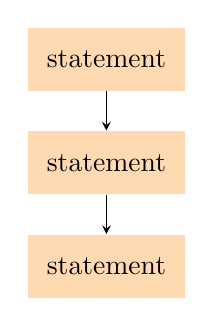
\begin{tikzpicture}[node distance=0,
  process/.style = {rectangle, minimum width=2cm, minimum height=.8cm,
    text centered, fill=orange!30},
  decision/.style = {diamond, minimum width=2cm, minimum height=.8cm,
    text centered, fill=green!30, inner sep=0},
  flow/.style = {draw,->,>=stealth}]

  \node [process] (s0) {statement};
  \node [process, below=.5cm of s0] (s1) {statement};
  \node [process, below=.5cm of s1] (s2) {statement};

  \path [flow] (s0) -- (s1);
  \path [flow] (s1) -- (s2);

\end{tikzpicture}
\end{document}
